\section{Evaluation}
\label{s:results}

Our testbed experiments demonstrate that {\sword} delivers significant
performance boosts in terms of overall throughput and latency for
Clover. We discuss the relative impact of each of our techniques across
various workloads, and demonstrate that replacing compare-and-swap
requests with writes eliminates hardware bottlenecks.

\subsection{Testbed} 

\textbf{p4 testbed} Our testbed consists of 9 machines: a Clover memory server,
metadata server, and 7 Clover clients. Physically, the machines are identical:
each is equipped with two Intel Xeon E5-2640 CPUs and 256 GB of main memory
evenly spread across the NUMA domains. Each server is equipped with a Mellanox
ConnectX-5 100-Gbps NIC installed in a 16x PCIe slot, all of which are connected
to a 100-Gbps Edgecore Wedge-100 programable switch running
\sword.Figure~\ref{fig:overview} shows the layout of our testbed.


\textbf{dpdk testbed} Our testbed consists of three machines: a lock request
driver memory server, and a dpdk implementation of {\sword}.  Physically, the
machines are the same as above except they are connected to a 100-Gbps Mellanox
Onyx Switch. The lock request driver is are configured with default routing
settings: clients send directly to the memory servers. We install OpenFlow rules
on the Onyx switch to redirect the RDMA traffic to \sword; 

\subsection{Atomic replacement}

We show the ability of swapping compare-and-swap requests to writes to overcome
hardware atomic bottlenecks by running a micro-benchmark that focuses
exclusively on CAS performance. Specifically, we extract the CAS request alone
from Shermans's write operation and repeatedly generate it from one client to a
single memory server (while routing it through {\sword} as before).

%Here we remove clover from the
%mix and run a simple benchmark of RDMA CAS operations between two
%servers. \sword is routed to via a different set of OpenFlow rules.

Each client thread is bound to a its own queue pair, and all client
threads issue CAS requests to the same shared virtual address.  We
set the number of cores on the {\sword} middlebox to 24 so that in our maximal
test case each client thread flows through exactly one middlebox core
for the lowest degree of interference between QP.

%All requests are routed
%through our middlebox.
In the default case (labeled CAS in Figure~\ref{fig:cas_vs_swap}),
{\sword} lets CAS requests flow through without interference, each
on their own queue pair.  In the CAS$\rightarrow$Write configuration
{\sword} needs to rely upon the ordering semantics of RCs (because all
the requests are for the same memory address and therefore
conflict), so maps all client requests to the same QP at the server.
Due to DPDK queue-to-core partitioning requirements all TX for a
destination QP must be done by a specific core on the
middlebox. Because of this requirement all requests in this
configuration must flow through a single core prior to being issued to
the memory-side NIC.

%all client cores request the same address, and as such all are routed
%onto the same destination QP. Note that this configuration has the
%highest degree of contention for our middlebox as 24 client threads
%must be multiplexed to and from a single client connection. Further

\begin{figure}[t]
    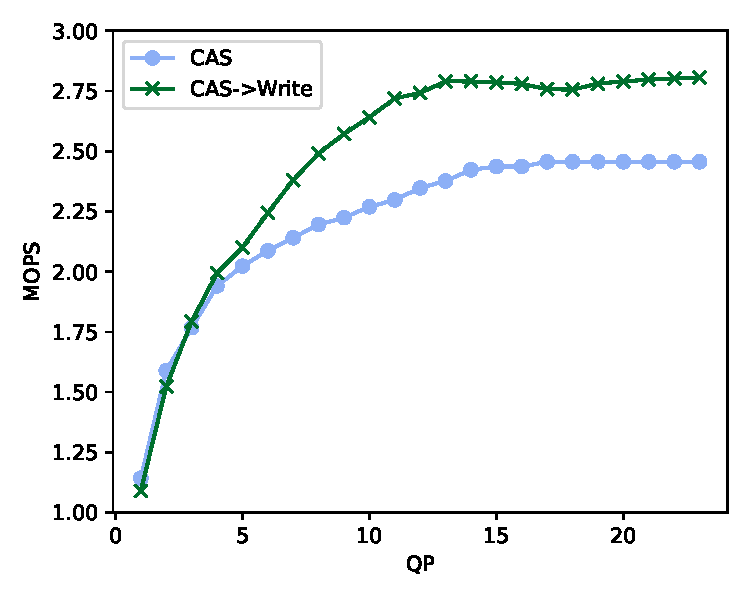
\includegraphics[width=0.485\textwidth]{fig/cas_vs_swap.pdf}
%  \vskip -0.5em
    \caption{Throughput of conflicting CAS and rewritten CAS requests as a function of client threads/QPs.}
    \label{fig:cas_vs_swap}
%      \vskip -0.5em
\end{figure}


We measure the server throughput in terms of RDMA requests per second as we
increase contention by adding client threads.  Figure~\ref{fig:cas_vs_swap}
shows the performance gained by converting CAS requests to writes. Both
configurations hit distinct bottlenecks: CAS requests bottleneck due to being
applied to a single key (c.f. Figure~\ref{fig:rdma_concur}). In the case of
converting CAS to write, the bottleneck is the processing power of the CPU cores
in our DPDK-based {\sword} prototype. (The maximum throughput our prototype can
process is 2.8 million requests per second per core.)
%In this configuration all requests to the memory server must be processed by
%the same TX core. As such our bottleneck is approximately 2.8 MOPS. Hardware
%implemented CRC, cache tuning, and better lock management for TX queues could
%yield higher per core performance in the future.
Despite this restriction, these results show that replacing CAS with write
avoids the memory server NIC's hardware bottleneck, enabling increased
scalability with a more performant {\sword}---such as one implemented on a
programmable switch. ~\sg{Our limitations here are due to programability issues
on the programmable switch, multiplexing across connections inflates state
reuqirements and makes storing dynamic connection state tricky given only a
static number of fixed width registers.}



\subsection{YCSB benchmarks}

\begin{figure*}
    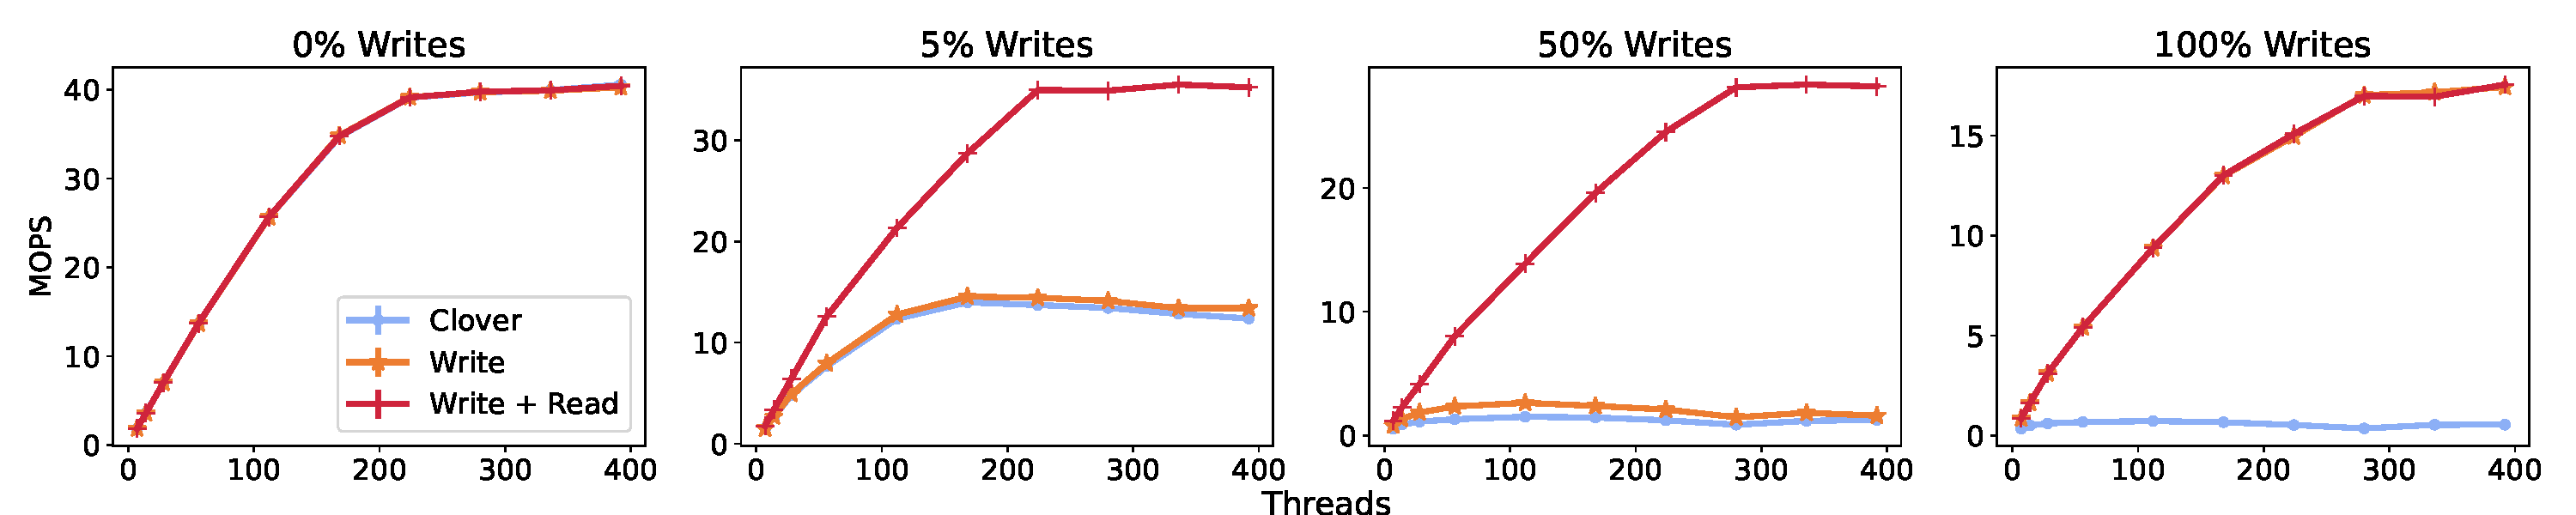
\includegraphics[width=1.0\textwidth]{fig/full_system_performance.pdf}
%  \vskip -0.5em
    \caption{{Performance of {\sword} techniques applied to Clover with 128 byte packets on 4 YCSB
    benchmarks. The percentage of workload writes increases from left to
    right. Our improvements over Clover are 1.0x, 2.8x, 32x, and 46x respectively.\todo{These are single runs not averages, rerun and capture error}}}
    \label{fig:full_system_performance}
      \vskip -0.5em
\end{figure*}

The YCSB benchmark consists of varying read and write workloads which
have been shown to emulate many common datacenter
operations~\cite{ycsb}. We show how \sword's read and write steering
improve the
%a
%breakdown of our techniques, mainly read and write caching, QP mapping, and
%atomic replacement with respect to their effect to system
performance on two
YCSB benchmarks. We choose YCSB-B (95\% read and 5\% write) as our baseline, and
YCSB-A (50\% read and 50\% write) to demonstrate how our algorithm performs
under high contention.  We also show the performance boosts obtained while
running a 100\% write workload which is intended to emulate other programmatic
workloads which are update heavy.

Figure~\ref{fig:full_system_performance} shows the relative
performance gains from each of \sword's techniques. At 5\% reads write
steering provides minimal performance improvement as the vast majority
of writes succeed on their first try. Individual writes, however, can
lead to many stale reads immediately thereafter which leads write steering
to offer a 1.17$\times$ throughput improvement.
%
%Applying QP mapping to the
%read majorly case adds too much computational overhead to give a
%benefit when writes are low, and only a few compare and swap
%operations exist.
%
At 50\% writes, Clover is well outside of it target workload:
at 64 threads, over half of all write requests fail. Here applying write
steering improves performance by over 1.73$\times$ at 64 threads.

Write steering alone is insufficient at this level of contention.
Because all writes succeed they easily out-pace reads causing the
majority of reads to fail at 64 threads.  (The resulting impact on
tail latency is clearly shown in Figure~\ref{fig:tail_latency}.)
Applying both read and write steering, on the other hand, yields a
2.82$\times$ throughput improvement as nearly all requests succeed.
%
%This workload leads to enough common case failures that
%performance overhead of performing QP mapping still yields a
%performance boost.
%
Write-only workloads are antagonistic to Clover's optimistic
approach: write and write+read steering yield 3.89$\times$ and
3.63$\times$ throughput improvements respectively; the read-steering
logic is pure overhead due to the absence of reads.
%in the workload.



%%\todo{real takeaways}

% \subsection{Memory Utilization}
% Our techniques give a performance boost at the cost of in network memory. We
% took special care to design our algorithms so that they could 1) use only a
% small amount of network memory, 2) be scalable depending on the resources
% available. We show how our performance varies as a function of the available in
% network state.

% As seen in Figure~\ref{fig:cache} our write caching is able to provide a
% significant performance boost while only using a small number of cached
% addresses. In the following experiment we show the maximum performance boost we
% can provide as a function of the available in network memory. Specifically in
% the case of read and write caching this means shrinking the size of the
% available cache. In terms of QP mapping it restricts the number of connections
% which can have their connections mapped. Unmapped connections must use atomic
% operations for their requests to succeed.

% \begin{figure}
%     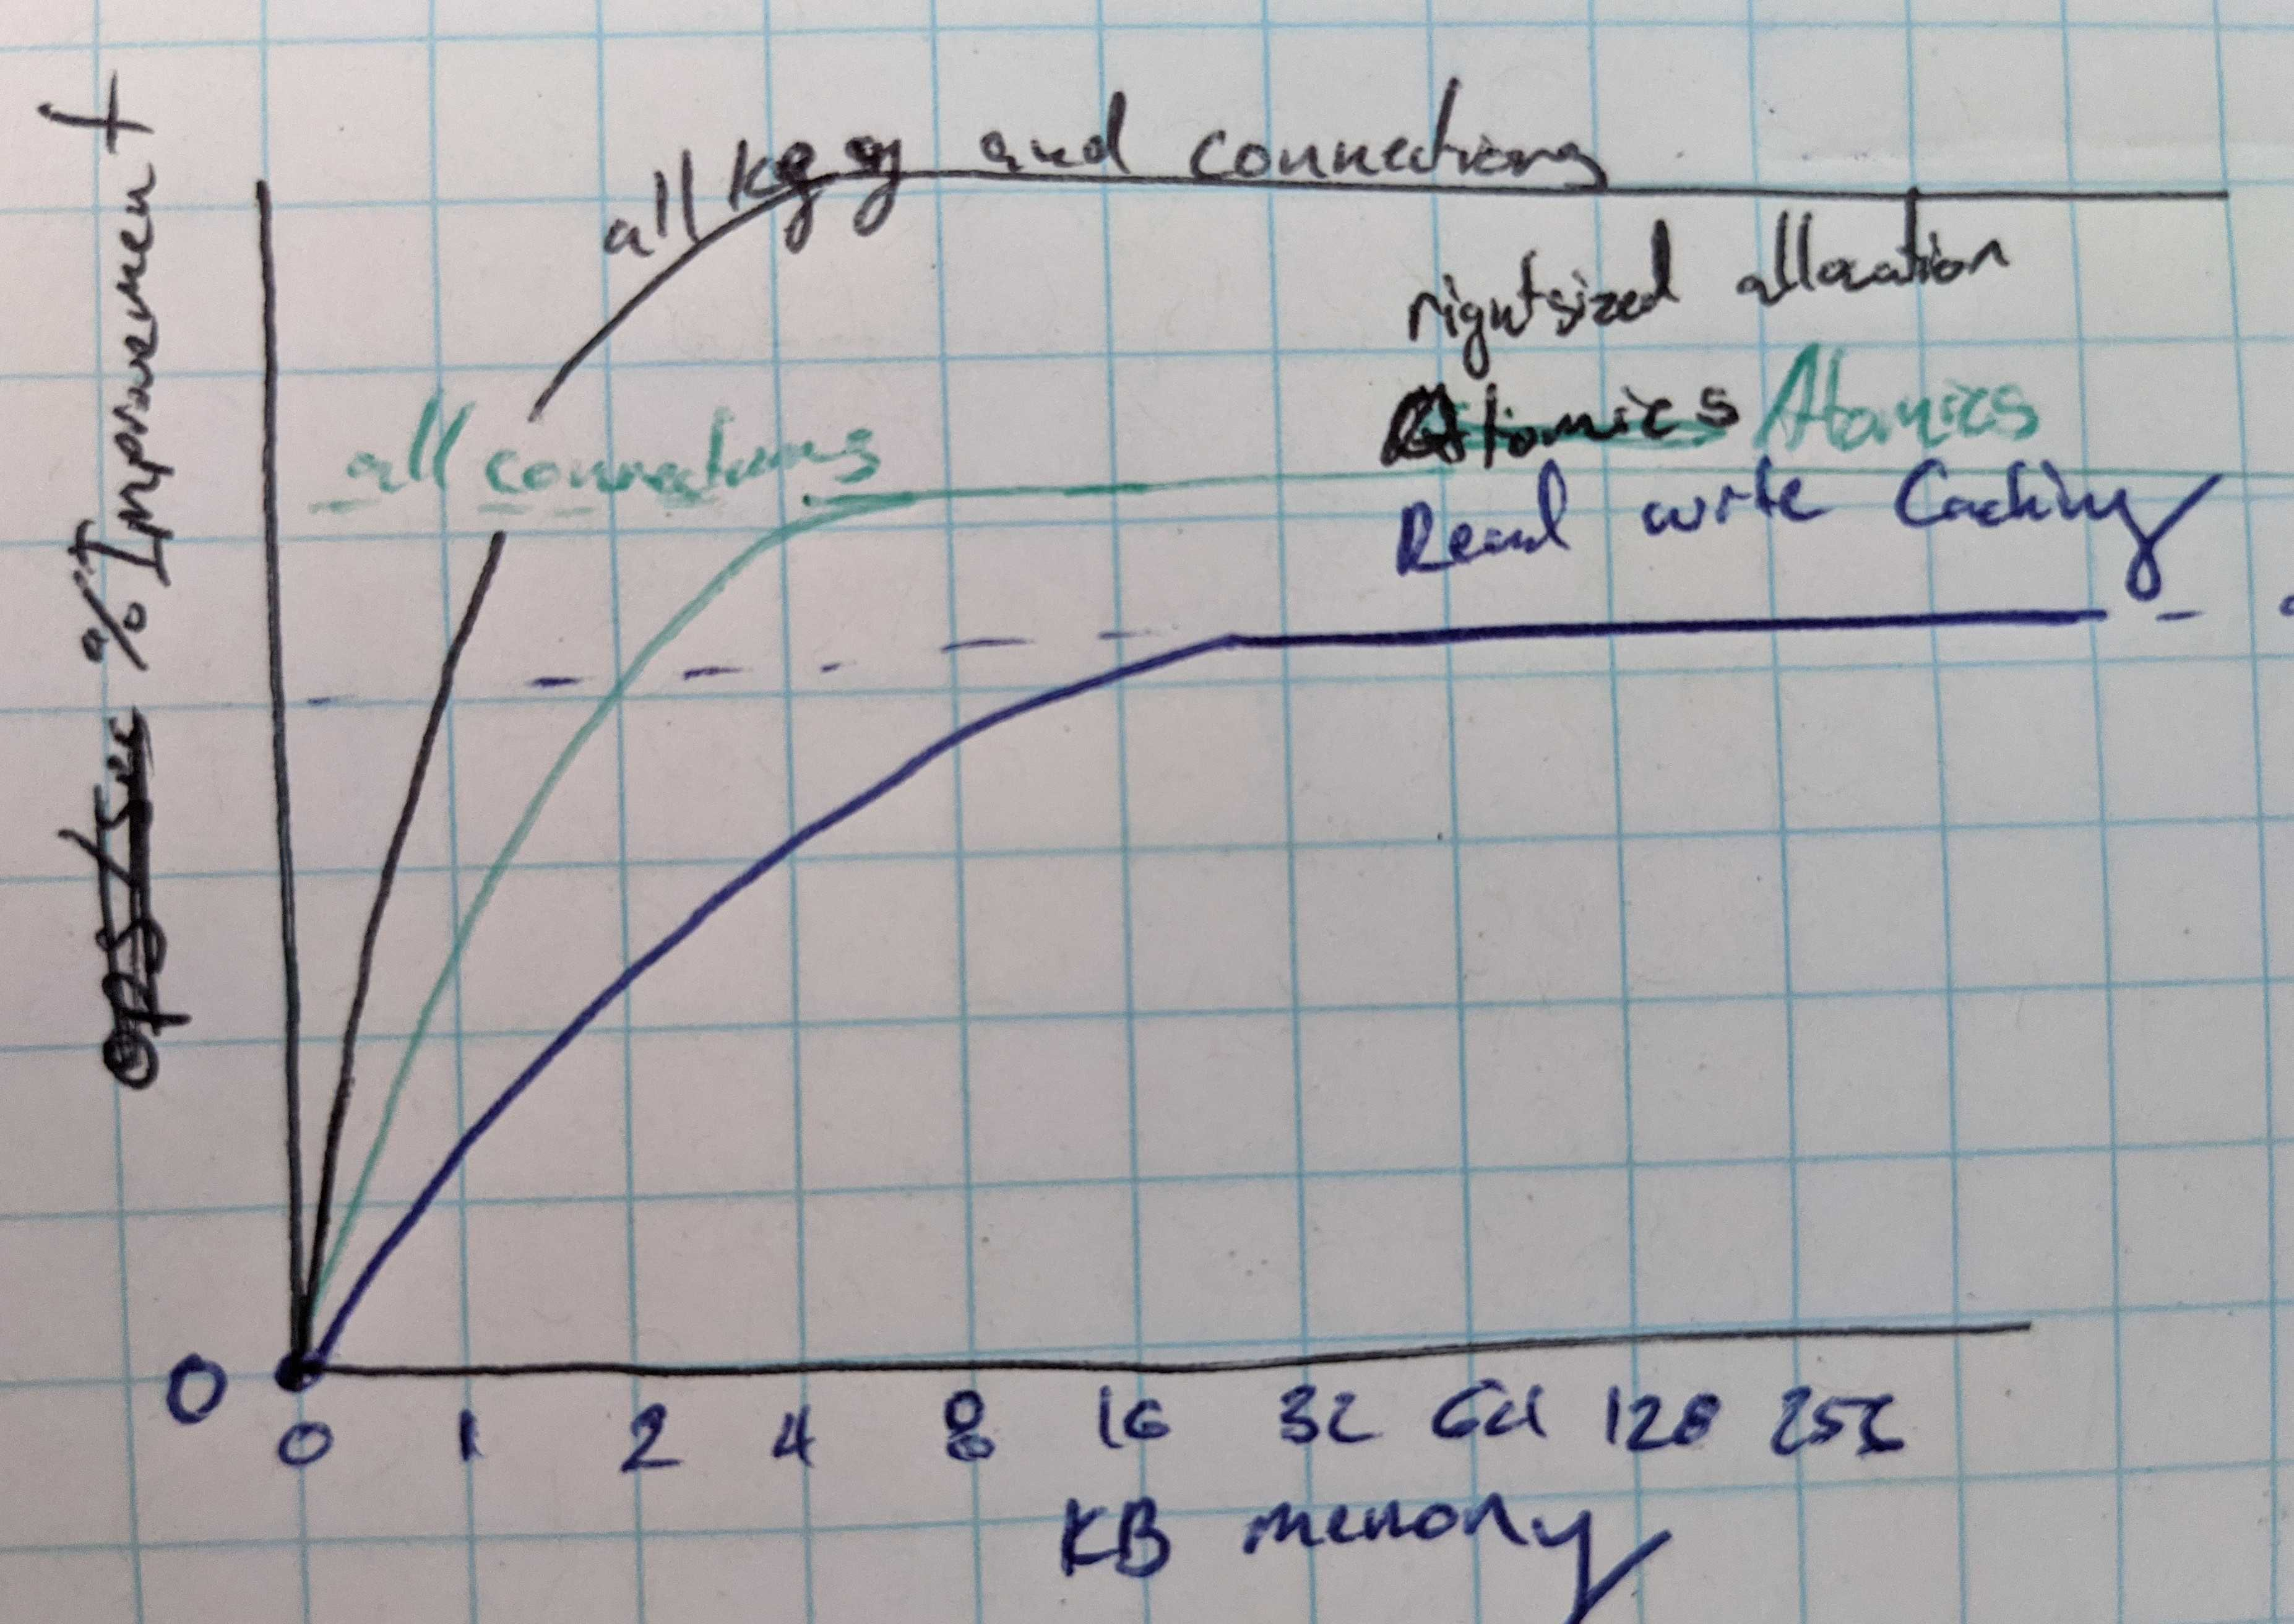
\includegraphics[width=0.45\textwidth]{fig/memory_util.jpg}
%     \caption{{Relative performance improvement of our techniques with restricted amounts of memory. Here a rightsized allocation implies that for the given number of connections we could support, all requests were mapped and reads and writes were cached.}}
%     \label{fig:memory_util}
% \end{figure}
%%\todo{say something real about the the memory utilization takeaways}


\subsection{Bandwidth reduction}

\begin{figure}
  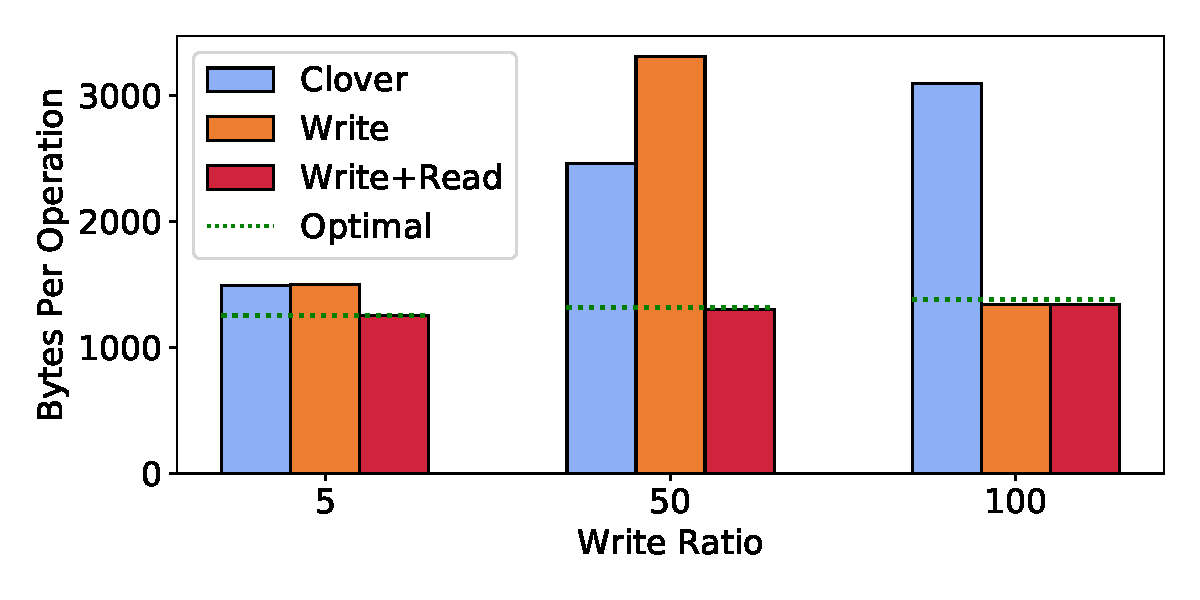
\includegraphics[width=0.485\textwidth]{fig/bandwidth_reduction.pdf}
  \centering
   \vskip -0.5em
    \caption{Bytes required per Clover operation on 128 byte payloads for each of the three techniques for different write intensities.}
    \label{fig:bandwidth_reduction}
     \vskip -0.5em
\end{figure}


\begin{figure}
    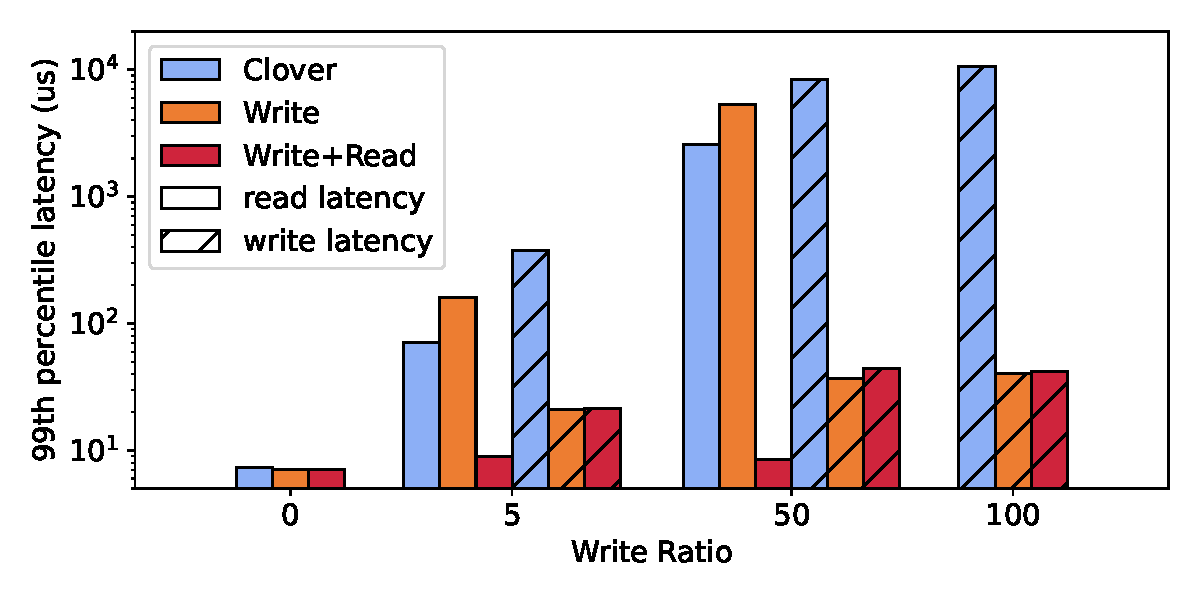
\includegraphics[width=0.485\textwidth]{fig/99th_latency_dense.pdf}
%\vskip -1em
    \caption{99th-percentile tail latencies of read (left) and write
      (right) Clover operations for workloads of various write
      intensities when applying each of {\sword}'s techniques.  Each
      measurement taken over a Zipf distribution of requests with 64
      clients. (Note the logarithmic $y$ axes.)}
    \label{fig:tail_latency}
      \vskip -0.5em
\end{figure}


Placing memory operations in-band with regular network traffic can be
problematic as applications' remote memory usage has the potential to
vary dramatically per application.  Under contention, memory operation
can require additional packet exchanges which inflate the bandwidth
necessary to service the same number of memory requests. Our
in-network steering algorithms remove the need for requests to
retry.

%Figure~\ref{fig:bandwidth_reduction} shows the average bytes
%per Clover operation under three different workloads for default
%Clover as well as {\sword}'s two steering techniques.

We calculate the optimal expected cost of a Clover operation by
averaging the cost of a successful operation across reads and
writes. We get the weighted average by multiplying the cost of a read
and write by the appropriate workload percentage. Each write consists
of an RDMA write followed by a CAS, along with the responses for each
message. A read consists of an RDMA read and read response, and
usually an additional metadata read made asynchronously with the main
read to fetch the latest position of the tail in case the first memory
read fails. Clover performs this second read opportunistically (in
around 99 percent of all reads in these workloads), however sometimes
it is omitted leading to a small over-approximation in our estimate of
``optimal''.

Figure~\ref{fig:bandwidth_reduction} show the average bytes per
operation for each strategy across all three write workloads. We
calculate the value for each technique by summing the total bandwidth
across a run and dividing by the total number of operations. Clover's
bandwidth usage increases with contention, growing by 1.8$\times$ at
50\% and 2.24$\times$ at 100\% writes---all of which is recovered by
applying read and write steering. Write steering alone causes
significant inflation in the cost of operations at 50\% writes because many
read requests fail as discussed above.

\subsection{Tail latency}

Perhaps the most critical variable that governs overall system
performance is tail latency. In the context of disaggregated memory
systems, reads and writes are often deeply integrated into the
computational logic of a program and the whole program must wait for a
page fault to complete before continuing. We therefore consider poor
tail latency to be a fundamental barrier to the widespread adoption of
far memory systems.  Optimistic concurrency is well known to exhibit
poor tail latency under contention, and Clover is no exception to this
rule. Our techniques significantly reduce latency as steering
ensures that nearly all requests succeed on the first try.

Figure~\ref{fig:tail_latency} shows the 99th-percentile tail latencies
associated with each of \sword's techniques in comparison with default
Clover. Clover's read latency (left-hand plot) at 5\% reads is
91~$\mu$s, around 7.5$\times$ its baseline our our testbed. With read
and write steering the tail latency of reads drops to 38~$\mu$s---a
2.3$\times$ improvement over Clover even in this low-contention
regime. At 50\% writes the performance increase is roughly double.  As
discussed above, in either case applying write steering alone actually
hurts performance, as it makes reads more likely to fail.
%read performance is improves by 2$\times$
%relative to Clover with the exception of write steering alone. When
%write steering is applied without the aid of read steering the writes
%quickly out-pace the reads, leading the vast majority of reads to fail
%on their first attempt.
Given that these tests were conducted with a
Zipf distribution across 64 cores it is highly likely that more than
one thread is writing to the hottest keys at any point during the
run. This leads some read requests to fail 10s of times before
succeeding.

%Because of this property we suggest
%that read and write steering be used in concert unless the workload is
%explicitly known.

Writes (right-hand side of Figure~\ref{fig:tail_latency}) perform
worse than reads under contention in default Clover. Write+read
steering provides a 2.7$\times$, 37.1$\times$, and 25.2$\times$
improvement in tail latency, respectively, across 5, 50, and 100\%
write workloads.  As one might expect, performing write steering alone
privledges writes over reads, dropping their tail latencies even
further---but likely insufficiently enough to make up for the dramatic
spike in read tail latency

Figure~\ref{fig:tail_latency} also shows the performance of queue pair
mapping and atomic replacement (CAS$\rightarrow$Write) when applied in addition
to write+read steering.  Because the requests are already likely to
succeed, there is no reason to expect any significant drop in tail
latency by vectoring the requests to a particular QP or removing the
CAS guard.  Rather, these plots show that the (significant) 
logic required in {\sword} to implement these functions result in only
marginal increase in tail latency relative to steering alone---and still
significantly outperforms Clover alone.

\subsection{Packet Size}
\todo{Write about packet sizes}

\begin{figure}
  \centering
  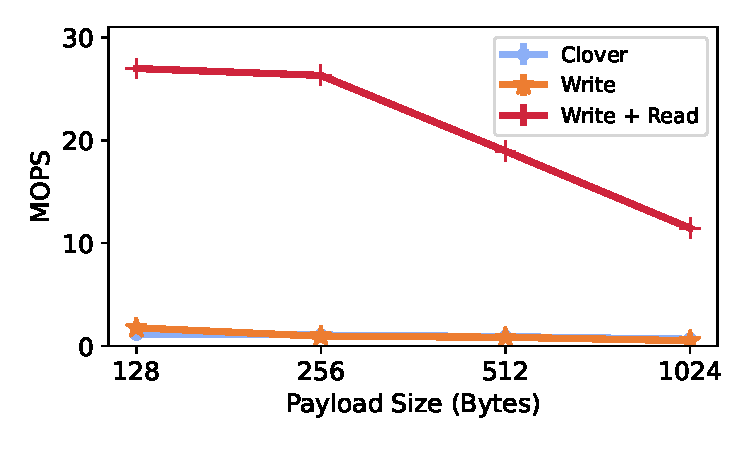
\includegraphics[width=0.485\textwidth]{fig/packet_size.pdf}

    \caption{Performance across RDMA payload sizes using 120 client cores at a 50 percent read 50 percent write ratio.}

    \label{fig:packet_size}
\end{figure}

\subsection{Contention}
\todo{Write about contention}
\begin{figure}
  \centering
  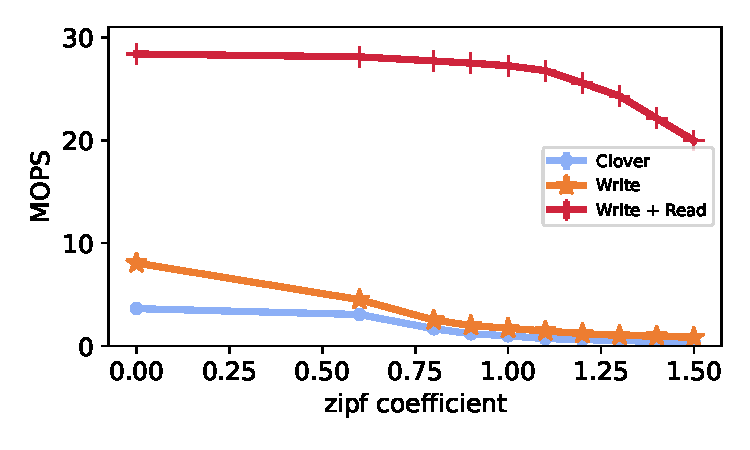
\includegraphics[width=0.485\textwidth]{fig/contention.pdf}

    \caption{Performance as contention increases with zipf coefficient using 120 client cores.
    \todo{These numbers need to be extended to 400 cores}}

    \label{fig:packet_size}
\end{figure}


%The application of QP mapping and swapping
%CNS to writes does little to effect tail latency as their performance
%cost comes largely as an increase to the average.


